Como en la sección anterior se ha logrado una implementación correcta de QAOA para un problema simple se continúa con un caso en el que se aplica el algoritmo a un problema distinto, con más qubits y con restricciones.

Estos resultados recopilados corresponden con el problema descrito en la \textit{sección~\ref{sec:4-primer_grafo}}, en el que se resuelve el problema del hallar el camino más corto entre los nodos 0{-}3 para el grafo de la \textit{figura~\ref{fig:4-primer_grafo}}.

\subsection{Resultados con QAOA}

\subsubsection{Solución del artículo\label{sec:5-primer-paper-resultados-qiskit}}
En las siguientes muestras se ha buscado replicar los resultados del \textit{artículo~\cite{multi-objective_routing_optimization}}, del que se ha obtenido el problema. Esto ha sido probado ya que, empleando los parámetros \(\beta = 0.28517317\) y \(\gamma = -5.05969577 \) dados como óptimos, se obtiene un gráfico muy similar al del artículo:

\begin{figure}[]{fig:5-primer-grafo/sin restriccion extra/primer paper aer resultado}{}
  \subfigure[]{Resultado del artículo}{
    \centering
    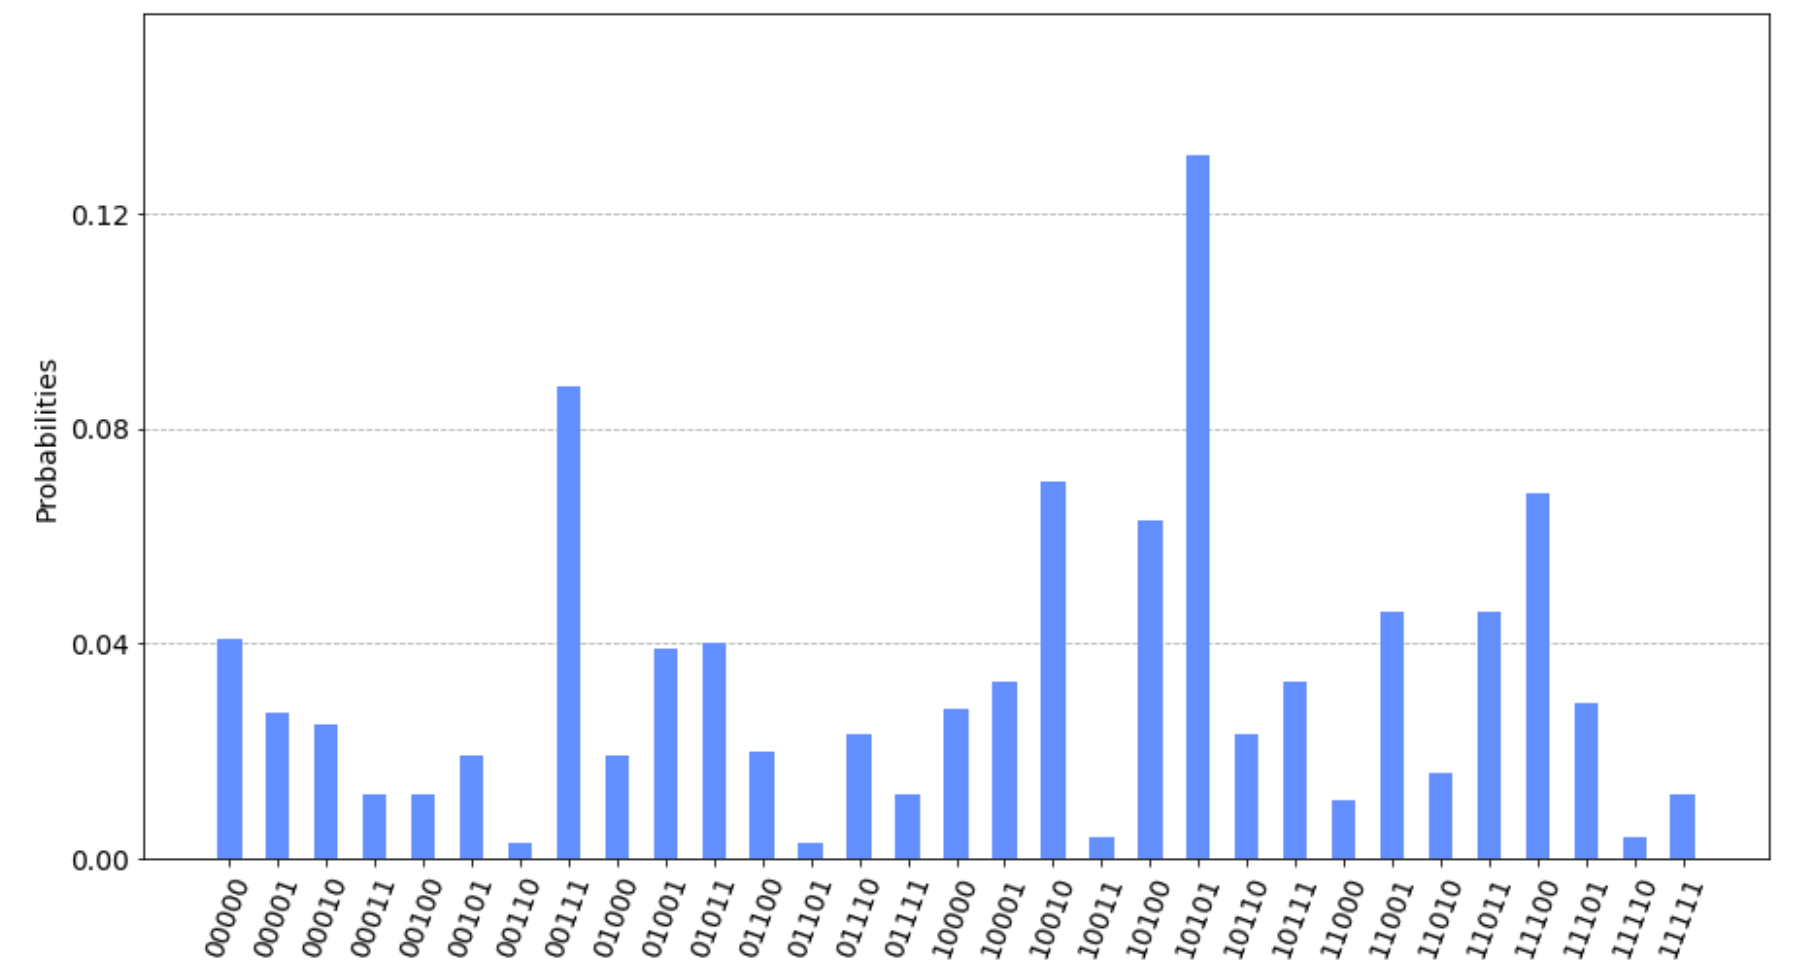
\includegraphics[width=0.42\textwidth]{primer-grafo/sin_restriccion_extra/primer_paper_orig_resultado}
  } \hfill
  \subfigure[]{Resultado obtenido}{
    \centering
    \includegraphics[width=0.49\textwidth]{primer-grafo/sin_restriccion_extra/primer_paper_aer_resultado}
  }
\end{figure}

De esta forma, se asume que los resultados del artículo deberían ser equivalentes a los obtenidos en esta instancia del algoritmo.

\begin{table}[htbp]{tab:5-primer-paper-aer_estadisticas}{Resultados de la ejecución de la versión de QAOA del artículo}
  \centering
  \begin{tabular}{|c|r|r|}
    \hline
    \textbf{nº Capas} & \textbf{Estadística máxima (\%)} & \textbf{Estadística global (\%)} \\ \hline
    p = 1             & 91.3\%                           & 39.34\%                          \\ \hline
    p = 2             & 64.6\%                           & 24.16\%                          \\ \hline
    p = 3             & 63.4\%                           & 18.82\%                          \\ \hline
    p = 4             &  9.4\%                           &  5.38\%                          \\ \hline
    p = 5             & 67.9\%                           & 19.45\%                          \\ \hline
    p = 6             & 29.8\%                           & 12.59\%                          \\ \hline
    p = 7             & 28.9\%                           &  9.12\%                          \\ \hline
    p = 8             & 36.7\%                           & 12.49\%                          \\ \hline
  \end{tabular}
\end{table}

El primer resultado a resaltar en la \textit{tabla~\ref{tab:5-primer-paper-aer_estadisticas}} es un empeoramiento de los resultados a medida que se aumenta el número de capas, lo cual es contrario a lo esperado teóricamente.

Además, la gran diferencia entre los resultados dados por la estadística máxima y la estadística global denotan una gran cantidad de ruido al ejecutar el algoritmo, lo cual se corrobora viendo los resultados de ejecuciones concretas, como los dados en la \textit{figura~\ref{fig:5-primer-grafo/sin restriccion extra/primer paper aer resultado}}.

El resultado de la función gamma es el siguiente:
\begin{figure}[htbp]{fig:5-primer_grafo/sin_restriccion_extra/primer_paper_p_27_gamma_fun}{Función gamma. Caso del artículo}
  \centering
  \includegraphics[scale=0.5]{primer-grafo/sin_restriccion_extra/primer_paper_p_27_gamma_fun}
\end{figure}

Se puede ver que existen un gran número de mínimos locales, lo cual dificulta la tarea del optimizador clásico. Esto se corrobora ya que, al emplear como parámetros iniciales $(\beta = 1.0, \gamma = 0.5)$, para $p = 1$ se obtiene el camino óptimo el 100\% de las ejecuciones.

Este proceso de inicializar los parámetros con valores concretos no sería una solución válida, ya que se trata de una metodología no automática en la que, para ejecutar correctamente el algoritmo, se necesitaría conocer antes su propio resultado. Además la ejecución correcta sucede para $p = 1$, pero al igual que el caso por defecto $(\beta = 1.0, \gamma = 1.0)$, no escala correctamente al aumentar el número de capas.

\subsubsection{Modificaciones a la solución del artículo}
Partiendo de la solución del artículo descrita en la \textit{sección~\ref{sec:5-primer-paper-resultados-qiskit}}, se han realizado cambios a la función de coste y a la construcción del circuito cuántico con el fin de encontrar el mejor resultado. Esto se ha realizado para poder comparar el rendimiento de la mejor solución encontrada con el rendimiento del algoritmo de Quantum Annealing de D-Wave.

Las modificaciones empleadas han sido las siguientes:

\paragraph{Ángulos correctos teóricamente}
Al construir el circuito, utilizar para los operadores lineales los ángulos obtenidos teóricamente, en lugar de los vistos en el artículo (discutido en la \textit{sección~\ref{sec:4-primer_grafo_diferencias_con_el_articulo}}).

Las estadísticas obtenidas en la \textit{tabla~\ref{tab:5-primer-mod_originales-aer_estadisticas}} no dan ningún resultado satisfactorio.
Se aprecia un comportamiento similar al visto en los resultados del grafo de la \textit{tabla~\ref{tab:5-zhiqiang-aer_estadisticas}} en cuanto a que se mejoran las estadísticas hasta las 3 capas y luego disminuyen.

\begin{table}[htbp]{tab:5-primer-mod_originales-aer_estadisticas}{Resultados de la ejecución de QAOA utilizando los ángulos obtenidos teóricamente}
  \centering
  \begin{tabular}{|c|r|r|}
    \hline
    \textbf{nº Capas} & \textbf{Estadística máxima (\%)} & \textbf{Estadística global (\%)} \\ \hline
    p = 1             &  0.5\%                           &  4.05\%                          \\ \hline
    p = 2             &  9.2\%                           &  5.83\%                          \\ \hline
    p = 3             & 54.8\%                           & 12.98\%                          \\ \hline
    p = 4             & 11.1\%                           &  7.00\%                          \\ \hline
    p = 5             &    6\%                           &  5.71\%                          \\ \hline
  \end{tabular}
\end{table}

La función gamma resultante se muestra en la \textit{figura~\ref{fig:5-primer-mod_originales-gamma_fun}}.
Tiene un mínimo global menos claro con respecto a la función gamma de la versión del grafo del paper, en la \textit{figura~\ref{fig:5-primer_grafo/sin_restriccion_extra/primer_paper_p_27_gamma_fun}}.
Además a diferencia de dicha gráfica, en esta no se aprecia periodicidad alguna.

\begin{figure}[htbp]{fig:5-primer-mod_originales-gamma_fun}{Función gamma. Con ángulos correctos teóricamente.}
  \centering
  \includegraphics[scale=0.5]{primer-grafo/sin_restriccion_extra/primer-paper-mod_originales-gamma_fun}
\end{figure}

\paragraph{P=40}
% TODOOO: Repetir estas ejecuciones y hacer función gamma, por ahora salen demasiado mal como para mostrarlas
Incrementar el valor del parámetro P (correspondiente al modificador de Lagrange)
% TODO: Citar multiplicador de lagrange del anexo
al construir la función de coste, para así aumentar la penalización en caso de fallo.

\paragraph{Restricción extra}
Añadir una restricción a la función de coste, que especifique que solo se puede acceder al último nodo por una de las aristas que lleguen a este.
% TODOO: Esto seguramente no se explique aquí, en algún sitio hablar sobre la restricción extra. SI SE QUITA LA FORMULA QUITARLA DE LA CITA DE LA TABLA DE ABAJO

\begin{align}\label{eq:5-primer-restriccion_extra}
  X_{13} + X_{23} = 1
\end{align}

\begin{table}[htbp]{tab:5-primer-restriccion_extra-aer_estadisticas}{Resultados de la ejecución de QAOA añadiendo la restricción de la \textit{fórmula~\ref{eq:5-primer-restriccion_extra}}}
  \centering
  \begin{tabular}{|c|r|r|}
    \hline
    \textbf{nº Capas} & \textbf{Estadística máxima (\%)} & \textbf{Estadística global (\%)} \\ \hline
    p = 1             & 93.8\%                           & 37.83\%                          \\ \hline
    p = 2             & 64.6\%                           & 26.16\%                          \\ \hline
    p = 3             & 84.8\%                           & 27.82\%                          \\ \hline
    p = 4             & 56.0\%                           & 23.47\%                          \\ \hline
    p = 5             & 88.1\%                           & 46.40\%                          \\ \hline
    p = 6             & 88.1\%                           & 21.83\%                          \\ \hline
  \end{tabular}
\end{table}

Los resultados (\textit{tabla~\ref{tab:5-primer-restriccion_extra-aer_estadisticas}}) presentan una ligera mejora con respecto a los presentes en la \textit{tabla~\ref{tab:5-primer-paper-aer_estadisticas}}, tanto para las estadísticas máximas como globales.

La función gamma resultante (\textit{figura~\ref{fig:5-primer_grafo/con_restriccion_extra/primer_restr_aer_gamma_fun}}) toma, en comparación con la original (\textit{figura~\ref{fig:5-primer_grafo/sin_restriccion_extra/primer_paper_p_27_gamma_fun}}), unos valores elevados.
Se distingue un incremento en la diferencia entre los mínimos globales y los mínimos locales (no globales).

\begin{figure}[htbp]{fig:5-primer_grafo/con_restriccion_extra/primer_restr_aer_gamma_fun}{Función gamma. Con restricción extra}
  \centering
  \includegraphics[scale=0.5]{primer-grafo/con_restriccion_extra/primer_restr_aer_gamma_fun}
\end{figure}

\subsection{Resultados con QAOA en ordenador cuántico real}
Utilizando la herramienta Runtime de Qiskit se han realizado ejecuciones del código para comprobar sus resultados en ordenadores reales.

El funcionamiento ha consistido en obtener los parámetros $\gamma$ y $\beta$ en dichos ordenadores y después ejecutar una vez más en un simulador para obtener el resultado al problema.

\subsubsection{\(p = 1\)}
El código ha sido ejecutando con el error encontrado en el artículo (\textit{sección~\ref{sec:4-primer_grafo_diferencias_con_el_articulo}}), tratando así de asemejarse a los resultados obtenidos en el mismo.

El resultado obtenido ha sido el siguiente:

\begin{verbatim}
    message: Optimization terminated successfully.
    success: True
     status: 1
        fun: 52.81120901157566
          x: [ 7.624e-01  4.636e-01]
       nfev: 30
      maxcv: 0.0
\end{verbatim}

Este mensaje es devuelto por el optimizador clásico \href{https://docs.scipy.org/doc/scipy/reference/generated/scipy.optimize.minimize.html}{scipy.optimize.minimize}
y significa que se han encontrado los parámetros $\gamma = 0.7624$ y $\beta = 0.4636$, con los que la función \textit{execute\_circuit} devuelve un valor de $52.81$. Esto está muy lejos de ser una media óptima, ya que esta se daría al obtener en todos los casos el camino más corto, lo que daría una media de 11 (el coste de dicho resultado).
El otro valor a remarcar, \textit{nfev=$30$}, se refiere al número de ejecuciones de la función \textit{execute\_circuit} realizadas.

Los parámetros obtenidos, ejecutados en un simulador, dan el siguiente resultado:
\begin{figure}[htbp]{fig:5-primer_grafo/sin_restriccion_extra/primer-runtime-mod_paper-1_capa-nairobi_aer}{Ejecución de $\gamma, \beta$ en simulador}
  \centering
  \includegraphics[scale=0.4]{primer-grafo/sin_restriccion_extra/primer-runtime-mod_paper-1_capa-nairobi_aer}
\end{figure}

Esto indica que el motivo de obtener un resultado inesperadamente alto de la función se debe a la presencia de un camino, \textit{10001}, de coste elevado obtenido un gran número de veces. Este camino es costoso, con valor de 63, debido a que rompe varias restricciones de la función de coste.

Estos mismos parámetros resultados de la ejecución en \textit{ibm\_nairobi} han sido ejecutados en el ordenador de \textit{ibm\_lagos}, dando los resultados de la \textit{figura~\ref{fig:5-primer_grafo/sin_restriccion_extra/primer-runtime-mod_paper-1_capa-nairobi_lagos}}.

\begin{figure}[htbp]{fig:5-primer_grafo/sin_restriccion_extra/primer-runtime-mod_paper-1_capa-nairobi_lagos}{Ejecución de \(\gamma, \beta\) en \textit{ibm\_lagos}}
  \centering
  \includegraphics[scale=0.4]{primer-grafo/sin_restriccion_extra/primer-runtime-mod_paper-1_capa-nairobi_lagos}
\end{figure}

Comparando las \textit{figuras~\ref{fig:5-primer_grafo/sin_restriccion_extra/primer-runtime-mod_paper-1_capa-nairobi_aer}} y\textit{~\ref{fig:5-primer_grafo/sin_restriccion_extra/primer-runtime-mod_paper-1_capa-nairobi_lagos}}
se aprecia la diferencia de ejecutar unos mismos parámetros en un simulador y un ordenador cuántico real. Aunque los resultados sean similares el número de ocurrencias de la cadena de bits correspondiente con el camino óptimo disminuye notablemente en la ejecución real, debido al ruido presente en toda ejecución de un circuito cuántico.


\subsection{Resultados de D-Wave}

Con respecto a los resultados de aplicar Quantum Annealing utilizando los sistemas de D-Wave se ha obtenido el resultado de la \textit{tabla~\ref{tab:5-primer-dwave_estadisticas}}

\begin{table}[htbp]{tab:5-primer-dwave_estadisticas}{Resultados de la ejecución del camino más corto en grafo de 4 nodos en D-Wave}
  \centering
  \begin{tabular}{|c|r|r|}
    \hline
    \textbf{Camino}         & \textbf{Energía} & \textbf{Número de ocurrencias} \\ \hline
    10101 (\textbf{Óptimo}) & 11               & 348                            \\ \hline
    10010                   & 12               & 373                            \\ \hline
    01001                   & 12               & 294                            \\ \hline
    00000                   & 54               &   4                            \\ \hline
    10000                   & 58               &   1                            \\ \hline
    00001                   & 59               &   1                            \\ \hline
    10100                   & 60               &   1                            \\ \hline
    00101                   & 61               &   1                            \\ \hline
    01010                   & 69               &   1                            \\ \hline
  \end{tabular}
\end{table}

La energía se refiere al coste de dicho camino de acuerdo con la función de coste utilizada. Se puede ver cómo, aunque se encuentre el camino óptimo un menor número de veces que en QAOA, existe una mayor coherencia en los resultados. Esto es así porque los caminos con mayores ocurrencias son los que tienen menor energía, mientras en las ejecuciones de Qiskit se pueden ver ejemplos, como es el camino 00111 en la \textit{figura~\ref{fig:5-primer-grafo/sin restriccion extra/primer paper aer resultado}} con un gran número de ocurrencias pero también una energía elevada.
\footnote{Con la formulación del problema dada, la energía del camino ``00111'' es 150. Esto se debe a que se rompen varias restricciones presentes en la función de coste. Este valor puede variar dependiendo del multiplicador de Lagrange empleado
  % TODO: Citar multiplicador de lagrange del anexo
  y las restricciones utilizadas.}


\subsection{Resultados con librería de QAOA}

En la siguiente sección se muestran unas estadísticas calculadas en la implementación de QAOA de la librería de Qiskit, \textit{QAOAAnsatz}.
Se utilizará para comparar con la implementación propia de QAOA, para así poder asegurarse de que el funcionamiento es el esperado.
La función mencionada, \textit{QAOAAnsatz}, construye un circuito a partir de un hamiltoniano, que en este caso será equivalente al operador \textit{C} correspondiente al \textbf{problem hamiltonian}.

\begin{table}[htbp]{}{Resultados utilizando \textit{QAOAAnsatz} con el problema de la \textit{figura~\ref{fig:4-primer_grafo}}}
  \centering
  \begin{tabular}{|c|r|r|}
    \hline
    \textbf{nº Capas} & \textbf{Estadística máxima (\%)} & \textbf{Estadística global (\%)} \\ \hline
    p = 1             &  1.0\%                           &  5.54\%                          \\ \hline
    p = 2             &  5.0\%                           &  4.58\%                          \\ \hline
    p = 3             & 47.0\%                           & 12.36\%                          \\ \hline
    p = 4             &  1.0\%                           &  6.91\%                          \\ \hline
    p = 5             &  5.0\%                           &  6.34\%                          \\ \hline
  \end{tabular}
\end{table}

Comparando la tabla generada con la \textit{tabla~\ref{tab:5-primer-mod_originales-aer_estadisticas}} se puede ver que son muy similares.
Esto garantiza que la implementación del algoritmo desarrollada en la \textit{sección~\ref{sec:4-primer_grafo}} es correcta.
También, se apoya la hipótesis de que los cálculos seguidos en el artículo del que se ha obtenido el problema (artículo~\cite{multi-objective_routing_optimization}) son incorrectos (resultados de la tabla~\ref{tab:5-primer-paper-aer_estadisticas}).


%%% Local Variables:
%%% mode: latex
%%% TeX-master: "../tfgtfmthesisuam"
%%% End:
